\documentclass[a4paper,11pt]{article}
\usepackage[utf8]{inputenc}
\usepackage{graphicx}
\usepackage{enumerate}
\usepackage{geometry}
\usepackage{fancyhdr}
\usepackage{minted}
\usepackage{xcolor}
\usepackage{listings}
\usepackage[colorlinks = true,
            linkcolor = blue,
            urlcolor  = blue,
            citecolor = blue]{hyperref}

\geometry{total={210mm,297mm},
left=25mm,right=25mm,%
bindingoffset=0mm, top=20mm,bottom=20mm}

\graphicspath{ {./images/} }
\renewcommand{\thesubsubsection}{\thesubsection.\alph{subsubsection}}
\renewcommand*\sfdefault{phv}
\renewcommand\familydefault{\sfdefault}

% \renewcommand{\thesubsubsection}{\thesubsection.\alph{subsubsection}}

% \newmintedfile{html}{
%     linenos,
%     breaklines,
%     python3,
%     numbersep=8pt,
%     frame=single,
%     framesep=3mm} 

\newcommand*{\TitleFont}{%
      \usefont{\encodingdefault}{\rmdefault}{b}{n}%
      \fontsize{16}{20}%
      \selectfont}

\linespread{1.3}

% my own titles
\makeatletter
\renewcommand{\maketitle}{
\begin{center}
\vspace{2ex}
{\huge \textsc{\@title}}
\vspace{1ex}
\\
\rule{\linewidth}{0.5pt}\\
\@author \hfill \@date
\vspace{4ex}
\end{center}
}
\makeatother

\definecolor{bg}{rgb}{0.95,0.95,0.95}


% custom footers and headers
\pagestyle{fancy}
\lhead{}
\chead{}
\rhead{}
\lfoot{Assignment 7 : MTA(2) }
\cfoot{}
\rfoot{Page \thepage}
\renewcommand{\headrulewidth}{0pt}
\renewcommand{\footrulewidth}{0pt}
%%----------%%%----------%%%----------%%%----------%%%

\begin{document}

\newminted{bash}{fontsize=\scriptsize, 
    linenos,
    breaklines,
    python3,
    numbersep=8pt,
    frame=single,
    bgcolor=bg,
    framesep=3mm} 



% \newminted{all}{linenos, frame=single}

% \usemintedstyle{monokai}
\usemintedstyle{manni}
% \usemintedstyle{xcode}
% \usemintedstyle{vs}
% \usemintedstyle{autumn}
% \usemintedstyle{colorful}
% \usemintedstyle{trac}


\title{ \TitleFont Assignment 7 : MTA(2) }

\author{Emil Sharifulllin, Innopolis University}

\date{\today}

\maketitle

\tableofcontents

\section{Mailing Loops}
\subsection{Now send an email to the loop using your own email address and see what happens on your MTA.}
With my groumates I made a loop. To do this I created new alias in /etc/aliases

\begin{bashcode*}{label=/etc/aliases}
root: postfix 
e.sharifullin: postfix
litleleprikon: posfix
postmaster: postfix
loop: loop@st14.os3.su
\end{bashcode*}

\begin{bashcode*}{label=Message that has been looped}
From MAILER-DAEMON  Fri Oct  7 15:11:18 2016
Return-Path: <>
X-Original-To: root@st10.os3.su
Delivered-To: root@st10.os3.su
Received: by st10.os3.su (Postfix)
  id 182E0236F; Fri,  7 Oct 2016 15:11:18 +0000 (UTC)
Date: Fri,  7 Oct 2016 15:11:18 +0000 (UTC)
From: MAILER-DAEMON@st10.os3.su (Mail Delivery System)
Subject: Undelivered Mail Returned to Sender
To: root@st10.os3.su
Auto-Submitted: auto-replied
MIME-Version: 1.0
Content-Type: multipart/report; report-type=delivery-status;
  boundary="EC6C22373.1475853078/st10.os3.su"
Message-Id: <20161007151118.182E0236F@st10.os3.su>

This is a MIME-encapsulated message.

--EC6C22373.1475853078/st10.os3.su
Content-Description: Notification
Content-Type: text/plain; charset=us-ascii

This is the mail system at host st10.os3.su.

I'm sorry to have to inform you that your message could not
be delivered to one or more recipients. It's attached below.

For further assistance, please send mail to postmaster.

If you do so, please include this problem report. You can
delete your own text from the attached returned message.

                   The mail system

<loop@st10.os3.su>: mail forwarding loop for loop@st10.os3.su

--EC6C22373.1475853078/st10.os3.su
Content-Description: Delivery report
Content-Type: message/delivery-status

Reporting-MTA: dns; st10.os3.su
X-Postfix-Queue-ID: EC6C22373
X-Postfix-Sender: rfc822; root@st10.os3.su
Arrival-Date: Fri,  7 Oct 2016 15:11:17 +0000 (UTC)

Final-Recipient: rfc822; loop@st10.os3.su
Original-Recipient: rfc822;loop@st10.os3.su
Action: failed
Status: 5.4.6
Diagnostic-Code: X-Postfix; mail forwarding loop for loop@st10.os3.su

--EC6C22373.1475853078/st10.os3.su
Content-Description: Undelivered Message
Content-Type: message/rfc822

Return-Path: <root@st10.os3.su>
Received: by st10.os3.su (Postfix, from userid 1001)
  id EC6C22373; Fri,  7 Oct 2016 15:11:17 +0000 (UTC)
DKIM-Filter: OpenDKIM Filter v2.10.3 st10.os3.su EC6C22373
DKIM-Signature: v=1; a=rsa-sha256; c=relaxed/relaxed; d=st10.os3.su; s=mail;
  t=1475853077; bh=t4gNfqbMV9ANitv/Xd6vRgAiMUJxDttiSzF0Ta37TbA=;
  h=Date:From:From;
  b=CjGkK3eQLTqu62tfTcc54i1Gk0LRlpVJWoVnkfmTdNS+/Otc+uWDIsfBXjCBT7+Lg
   +3cme/nnpSUiR3VDtegj0htCjFgrrPCDcoNn58GyC7coB2f0qayU1B/jn2CLyLZwRB
   U5rwo/HlGe7lBkDT+TgDUZvJPYIS3Re7DXA114z0=
X-Spam-Checker-Version: SpamAssassin 3.4.1 (2015-04-28) on 2b3c9230e793
X-Spam-Level: ****
X-Spam-Status: No, score=4.3 required=6.0 tests=MISSING_HEADERS,
  MISSING_SUBJECT,RDNS_NONE,T_DKIM_INVALID autolearn=no autolearn_force=no
  version=3.4.1
Received: from st14.os3.su (unknown [188.130.155.47])
  by st10.os3.su (Postfix) with ESMTP id 97893236F
  for <loop@st10.os3.su>; Fri,  7 Oct 2016 15:11:17 +0000 (UTC)
Received: from st10.os3.su ([188.130.155.43])
  by st14.os3.su (8.15.2/8.15.2/Debian-3) with ESMTP id u97FBBPv014270
  for <loop@st14.os3.su>; Fri, 7 Oct 2016 20:11:12 +0500
Authentication-Results: st14.os3.su;
  dkim=pass (1024-bit key; unprotected) header.d=st10.os3.su header.i=@st10.os3.su header.b=PgPLetXG;
  dkim=fail reason="signature verification failed" (1024-bit key) header.d=st10.os3.su header.i=@st10.os3.su header.b=+qVjMvtK;
  dkim-atps=neutral
Received: by st10.os3.su (Postfix)
  id 8DF8D236F; Fri,  7 Oct 2016 15:11:05 +0000 (UTC)
Delivered-To: loop@st10.os3.su
Received: by st10.os3.su (Postfix, from userid 1001)
  id 796722373; Fri,  7 Oct 2016 15:11:05 +0000 (UTC)
DKIM-Filter: OpenDKIM Filter v2.10.3 st10.os3.su 796722373
DKIM-Signature: v=1; a=rsa-sha256; c=relaxed/relaxed; d=st10.os3.su; s=mail;
  t=1475853065; bh=t4gNfqbMV9ANitv/Xd6vRgAiMUJxDttiSzF0Ta37TbA=;
  h=Date:From:From;
  b=PgPLetXG+uz5ihfA2XOncFkKu9OntLG6Ivl2EgULSnfDnaQqcEwmQU3fASf2EBNo5
   1sgjBnWSMPG+WvsnSVHEPTOppw2vopv3YVnLMstmoDYSQEfZ5XNmdHphv1XzrqUAwU
   Q+E4uhbTuZZdU1epiB9Zkg9+yIRB3IBWCRZgUzrA=
Received: from st14.os3.su (unknown [188.130.155.47])
  by st10.os3.su (Postfix) with ESMTP id 131C72370
  for <loop@st10.os3.su>; Fri,  7 Oct 2016 15:11:05 +0000 (UTC)
Received: from st10.os3.su ([188.130.155.43])
  by st14.os3.su (8.15.2/8.15.2/Debian-3) with ESMTP id u97FB0Bv014262
  for <loop@st14.os3.su>; Fri, 7 Oct 2016 20:11:01 +0500
Received: by st10.os3.su (Postfix, from userid 0)
  id 66EAE2370; Fri,  7 Oct 2016 15:10:55 +0000 (UTC)
DKIM-Filter: OpenDKIM Filter v2.10.3 st10.os3.su 66EAE2370
DKIM-Signature: v=1; a=rsa-sha256; c=relaxed/relaxed; d=st10.os3.su; s=mail;
  t=1475853055; bh=j+uJ1+KwQjMpdNiCngwvlv2FTzZnzkokoCYASnN36NE=;
  h=Date:From:From;
  b=+qVjMvtKwFuvbbq3NkXxRUuXzGW0epJL6GROtDIf6bOPwn8A/3ED5dYi3Pv20m1rX
   zMzNshgM3a1isnh6O5nl8OWBpwfllu9OczGIhpW+4KlBF7Y2az1WmlsHX+b7BB/gEZ
   ycIZDUUBTSJqiomFiwdhuXaA+2ULpmaOgDDbAJAs=
Message-Id: <20161007151055.66EAE2370@st10.os3.su>
Date: Fri,  7 Oct 2016 15:10:51 +0000 (UTC)
From: root@st10.os3.su (root)
MIME-Version: 1.0
X-yoursite-MailScanner: Found to be clean, Found to be clean
X-yoursite-MailScanner-SpamScore: ssss, ssss
X-yoursite-MailScanner-Information: Please contact the ISP for more information
X-yoursite-MailScanner-ID: u97FBBPv014270
X-yoursite-MailScanner-From: root@st10.os3.su

Hi

-- 
This message has been scanned for viruses and
dangerous content by MailScanner, and is
believed to be clean.
\end{bashcode*}

\subsection{Can you change the behaviour of your MTA in response to this loop?}
When my MTA receives mail it searches in aliases db where to store or resend message. When postfix understands that message came to it second time it frop this mail and send to mail sender another mail with error message. The number of loops that postfix can allow can be defined with hopcount\_limit parameter.

\section{Virtual Domains}
\addtocounter{subsection}{3}
\subsubsection{Create a new subdomain within your domain and add an MX entry to it.}
To create a new subdomain I added following line to my zone file
\begin{bashcode*}{label=/etx/named/st10.os3.su}
...
mta   IN  MX  10  mail
...
\end{bashcode*}

\subsubsection{Then extend your MTA configuration to handle virtual domains, and have it also handle the email for the newly created domain.}
To implement this I added changed main.cf, /etc/postfix/vmailbox and then ran postmap /etc/postfix/vmailbox and postfix reload

\begin{bashcode*}{label=/etc/postfix/main.cf}
virtual_mailbox_domains = mta.st10.os3.su
virtual_mailbox_base = /var/mail/virtual
virtual_mailbox_maps = hash:/etc/postfix/vmailbox
virtual_uid_maps = static:5000
virtual_gid_maps = static:5000
\end{bashcode*}

\begin{bashcode*}{label=/etc/postfix/vmailbox}
litleleprikon@mta.st10.os3.su mta/litleleprikon  
\end{bashcode*}

\begin{bashcode}
postmap /etc/postfix/vmailbox
postfix reload
\end{bashcode}

\subsubsection{Show how you test this.}
I sent mail to my virtual domain litleleprikon@mta.st10.os3.su and received this email:
\begin{bashcode*}{label=/var/mail/virtual/mta/litleleprikon}
From e.sharifullin@innopolis.ru  Fri Oct  7 16:00:49 2016
Return-Path: <e.sharifullin@innopolis.ru>
X-Original-To: litleleprikon@mta.st10.os3.su
Delivered-To: litleleprikon@mta.st10.os3.su
Received: by st10.os3.su (Postfix, from userid 1001)
  id 4859B23AC; Fri,  7 Oct 2016 15:53:43 +0000 (UTC)
X-Spam-Checker-Version: SpamAssassin 3.4.1 (2015-04-28) on 2b3c9230e793
X-Spam-Level: 
X-Spam-Status: No, score=-1.0 required=6.0 tests=ALL_TRUSTED,T_DKIM_INVALID
  autolearn=ham autolearn_force=no version=3.4.1
Received: from smtp.university.innopolis.ru (unknown [10.90.104.9])
  by st10.os3.su (Postfix) with ESMTP id 192A123A8
  for <litleleprikon@mta.st10.os3.su>; Fri,  7 Oct 2016 15:53:43 +0000 (UTC)
Content-Language: ru-RU
Content-Type: text/plain; charset="us-ascii"
Content-ID: <8F4203871EDEAE4DA93BD1C62047C81D@innopolis.ru>
Content-Transfer-Encoding: quoted-printable
DKIM-Signature: v=1; a=rsa-sha256; d=innopolis.ru; s=unimail1;
  c=simple/simple; t=1475855622; h=from:subject:to:date:message-id;
  bh=zkoQcLAhjnopmrDjf5fIX7liz2gEWaIe5yJg+a2BdLU=;
  b=hTfMgKdut1QaBxehqPWjxIfELwWLeNO/bF6525OglU1Vett+G1EicKhNovybD4MkYnkaaU1ga/W
  /iWiWeJr6CeTJ1nsrZeU/v6sP/H55cFeGbeuvm1i7yUZVhLvD1BBxBFlEIbJS/Njc5zwymHrE64Kv
  WPOiXtRxX2woJuNdaLDzleGsIe+7XY+tlhenE2GR/hNBbQuI/5z1nKzJKb9GaCdbGo2/fNB7gyIlU
  WVEyyfAsTtJHsgSSQheJYQ1PsgZX8mVAgeGnxTZZkYDdSoINsiYWpwTNI6pxFbki0t8zEaSIxavRn
  d6XZcTQlZMZJgY4pjxjndpRsECc4TlDw3hPQ==
From: Emil Sharifullin <e.sharifullin@innopolis.ru>
To: "litleleprikon@mta.st10.os3.su" <litleleprikon@mta.st10.os3.su>
Subject: Re: Virtual test
Thread-Topic: Virtual test
Thread-Index: AQHSILCikuavt0n77EGDuceqJJhro6Cc7qsAgAAAzwCAAALMAA==
Date: Fri, 7 Oct 2016 15:53:41 +0000
Message-ID: <58CBE545-6676-473D-AAAF-6AD618EF5285@innopolis.ru>
References: <B3C904E1-F4CE-45FE-B43E-8F46038CBBB7@innopolis.ru>
 <87C255CA-6E97-4A6A-A22A-A707D72DDEE4@innopolis.ru>
 <7109133E-D5FE-408D-B220-A6259F88CFD1@innopolis.ru>
In-Reply-To: <7109133E-D5FE-408D-B220-A6259F88CFD1@innopolis.ru>
Accept-Language: en-US, ru-RU
X-MS-Has-Attach:
X-MS-TNEF-Correlator:
x-ms-exchange-messagesentrepresentingtype: 1
x-ms-exchange-transport-fromentityheader: Hosted
x-originating-ip: [10.90.137.18]
MIME-Version: 1.0

dratuti
\end{bashcode*}

\section{SPAM and Security}
\addtocounter{subsection}{4}

\subsubsection{Write a small paragraph that highlights the advantages and disadvantages of SPF and DomainKeys Identified Mail (DKIM).}
SPF (Sender Policy Framework) is a DNS text entry which shows a list of servers that should be considered allowed to send mail for a specific domain. Incidentally the fact that SPF is a DNS entry can also considered a way to enforce the fact that the list is authoritative for the domain, since the owners/administrators are the only people allowed to add/change that main domain zone.\\
DKIM (DomainKeys Identified Mail) should be instead considered a method to verify that the messages' content are trustworthy, meaning that they weren't changed from the moment the message left the initial mail server. This additional layer of trustability is achieved by an implementation of the standard public/private key signing process. Once again the owners of the domain add a DNS entry with the public DKIM key which will be used by receivers to verify that the message DKIM signature is correct, while on the sender side the server will sign the entitled mail messages with the corresponding private key.

\subsubsection{What would you choose at a first glance and why?}
I chose DKIM because it provides mail signing and sender authority check but SPF provides only authority check.

\subsubsection{Configure your system to support one of the two. Your system must support it for both sending and receiving email. You might need additional software packages or patches.}

To add following steps:

\textbf{Instaling OpenDKIM}
\begin{bashcode}
apt install opendkim opendkim-tools
\end{bashcode}

\textbf{Keys generation}
\begin{bashcode}
mkdir /etc/opendkim/
opendkim-genkey -D /etc/opendkim/ -d st10.os3.su -s mail
\end{bashcode}

\textbf{Allow postfix to access keys}

\begin{bashcode}
chgrp opendkim /etc/opendkim/*
chmod g+r /etc/opendkim/*
gpasswd -a postfix opendkim
\end{bashcode}

\textbf{Configuring OpenDKIM}\\
To configure OpenDKIM I changed file /etc/opendkim.conf, keytable and signingtable  files.

\begin{bashcode*}{label=/etc/opendkim.conf}
Canonicalization relaxed/relaxed
Mode s
KeyTable file:/etc/opendkim/keytable
SigningTable file:/etc/opendkim/signingtable
SoftwareHeader yes
Socket inet:59909@localhost
\end{bashcode*}

\begin{bashcode*}{label=/etc/opendkim/keytable}
mail._domainkey.st10.os3.su st10.os3.su:mail:/etc/opendkim/mail.private 
\end{bashcode*}

\begin{bashcode*}{label=/etc/opendkim/signingtable}
st10.os3.su mail._domainkey.st10.os3.su 
\end{bashcode*}

\textbf{Configuring postfix}
\begin{bashcode}
postconf -e milter_default_action=accept
postconf -e milter_protocol=2
postconf -e smtpd_milters = inet:localhost:59909
postconf -e non_smtpd_milters = inet:localhost:59909
\end{bashcode}

\textbf{Restart services}
\begin{bashcode}
postfix reload
service opendkim start
\end{bashcode}

\subsubsection{Provide full email/MTA headers to prove that SPF/DKIM were implemented correctly on your system (sending and receiving).}
I sent email to my yandex mailbox
\begin{bashcode}
sendmail -t litleleprikon@yandex.ru
Hello
.
\end{bashcode}

This email I received in my yandex mailbox.

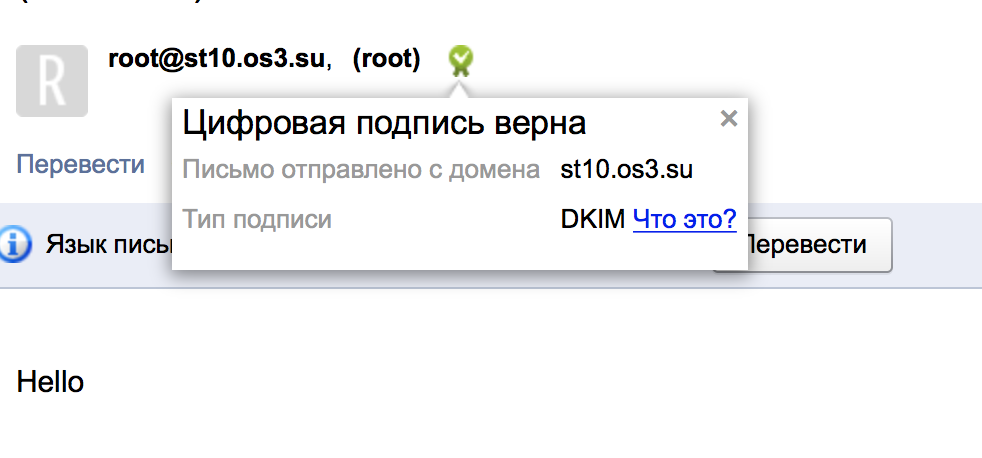
\includegraphics{mail_delivered}
\begin{bashcode}
Received: from mxfront3g.mail.yandex.net ([127.0.0.1])
  by mxfront3g.mail.yandex.net with LMTP id y9eMImzt
  for <litleleprikon@yandex.ru>; Thu, 29 Sep 2016 18:48:22 +0300
Received: from mail.st10.os3.su (mail.st10.os3.su [188.130.155.43])
  by mxfront3g.mail.yandex.net (nwsmtp/Yandex) with ESMTP id bWjHWXlA3f-mL2a04Bq;
  Thu, 29 Sep 2016 18:48:21 +0300
Return-Path: root@st10.os3.su
X-Yandex-Front: mxfront3g.mail.yandex.net
X-Yandex-TimeMark: 1475164101
To: undisclosed-recipients:;
Authentication-Results: mxfront3g.mail.yandex.net; dkim=pass header.i=@st10.os3.su
X-Yandex-Spam: 1
Received: by st10.os3.su (Postfix, from userid 0)
  id ABA12ADC; Thu, 29 Sep 2016 15:48:21 +0000 (UTC)
DKIM-Filter: OpenDKIM Filter v2.10.3 st10.os3.su ABA12ADC
DKIM-Signature: v=1; a=rsa-sha256; c=relaxed/relaxed; d=st10.os3.su; s=mail;
  t=1475164101; bh=Ba3gj8+xBPQLJTahTfzW6RbWQ/XPgESxkCi2B66PSQg=;
  h=Date:From:From;
  b=y1j0e9CsOTvcsIO3IaxjAeXPx+W7h2aDuog/fJDbIH9C5Sn2w18StnSerC/dMwgZZ
   0guvgzWvIu4wUY1WpbnCnN6MkLs7bvsDLLNqDQnQ2fgSQ7X/mdJSNviWWxVbrX+Wa/
   6SwtEZGbn5DDoJhRebb7zV+nyoTX7fJ4EctWuyhc=
Message-Id: <20160929154821.ABA12ADC@st10.os3.su>
Date: Thu, 29 Sep 2016 15:48:16 +0000 (UTC)
From: root@st10.os3.su (root)
X-Yandex-Forward: a9bfa178480f2904735134056b50d4a8

Hello
\end{bashcode}

\subsection{Investigate what generic anti-spam open source software packages are out there, choose one, download it (compile it if necessary) and configure your MTA to use it. Make sure that in your MTA group there are 2 different anti-spam solutions implemented!}
Main \href{http://www.postfix.org/addon.html}{site} of postfix MTA contains list of all anti-viruses and anti-spam solutions. For my pirposes I chose SpamAssassin as antispam solution.

To install SpamAssassin I typed this command:
\begin{bashcode}
$ apt-get install spamassassin spamc
\end{bashcode}

Next step is to create new user and setup access to directories.
\begin{bashcode}
$ groupadd spamd
$ useradd -g spamd -s /bin/false -d /var/log/spamassassin spamd
$ mkdir /var/log/spamassassin
$ chown spamd:spamd /var/log/spamassassin
\end{bashcode}
SpamAssassin have two config files: /etc/default/spamassassin that contains service configuration and /etc/spamassassin/local.cf that contains analisys preferences.
\begin{bashcode*}{label=/etc/default/spamassassin}
ENABLED=1
CRON=1
SAHOME="/var/log/spamassassin/"
OPTIONS="--create-prefs --max-children 2 --username spamd -H ${SAHOME} -s ${SAHOME}spamd.log"
\end{bashcode*}

\begin{bashcode*}{label=/etc/spamassassin/local.cf}
rewrite_header Subject [***** SPAM _SCORE_ *****]
required_score 6.0
use_bayes 1
bayes_auto_learn 1
\end{bashcode*}

After this manipulations we need to configure postfix 
\begin{bashcode*}{label=/etc/postfix/master.cf}
smtp      inet  n       -       -       -       -       smtpd -v -o content_filter=spamassassin

spamassassin unix -     n       n       -       -       pipe
 user=spamd argv=/usr/bin/spamc -f -e
 /usr/sbin/sendmail -oi -f ${sender} ${recipient}
\end{bashcode*}

Last step is to start services
\begin{bashcode}
$ postfix reload
$ service spamassassin start
\end{bashcode}

To test spam filter I sent special test message to my server and got mail marked as a spam.

\begin{bashcode*}{label=Test text}
XJS*C4JDBQADN1.NSBN3*2IDNEN*GTUBE-STANDARD-ANTI-UBE-TEST-EMAIL*C.34X
\end{bashcode*}

\begin{bashcode*}{label=Marked message}
From litleleprikon@gmail.com  Wed Oct  5 12:57:35 2016
Return-Path: <litleleprikon@gmail.com>
X-Original-To: litleleprikon@st10.os3.su
Delivered-To: litleleprikon@st10.os3.su
Received: by st10.os3.su (Postfix, from userid 1001)
        id 28BF01796; Wed,  5 Oct 2016 12:57:35 +0000 (UTC)
X-Spam-Checker-Version: SpamAssassin 3.4.1 (2015-04-28) on 2b3c9230e793
X-Spam-Flag: YES
X-Spam-Level: **************************************************
X-Spam-Status: Yes, score=1000.0 required=6.0 tests=FREEMAIL_FROM,GTUBE,
        HTML_MESSAGE,RCVD_IN_MSPIKE_H3,RCVD_IN_MSPIKE_WL,T_DKIM_INVALID autolearn=no
        autolearn_force=no version=3.4.1
X-Spam-Report:
        * 1000 GTUBE BODY: Generic Test for Unsolicited Bulk Email
        *  0.0 FREEMAIL_FROM Sender email is commonly abused enduser mail provider
        *      (litleleprikon[at]gmail.com)
        *  0.0 HTML_MESSAGE BODY: HTML included in message
        * -0.0 RCVD_IN_MSPIKE_H3 RBL: Good reputation (+3)
        *      [209.85.215.44 listed in wl.mailspike.net]
        * -0.0 RCVD_IN_MSPIKE_WL Mailspike good senders
        *  0.0 T_DKIM_INVALID DKIM-Signature header exists but is not valid
Received: from mail-lf0-f44.google.com (mail-lf0-f44.google.com [209.85.215.44])
        by st10.os3.su (Postfix) with ESMTP id AFBC71794
        for <litleleprikon@st10.os3.su>; Wed,  5 Oct 2016 12:57:34 +0000 (UTC)
Received: by mail-lf0-f44.google.com with SMTP id b75so77846240lfg.3
        for <litleleprikon@st10.os3.su>; Wed, 05 Oct 2016 05:57:34 -0700 (PDT)
DKIM-Signature: v=1; a=rsa-sha256; c=relaxed/relaxed;
        d=gmail.com; s=20120113;
        h=from:mime-version:subject:message-id:date:to;
        bh=ElHgS1JythLjtPMYUxcGlK6T9pka1f5adn84+vbvskc=;
        b=voaSK+Nd9W5Y6Cj0BctlIZEWnNGSvcvp91mn/rHXwsngcObdGnGJW958YqBvR8zCqX
         4BdDtK725ErPbu3PvU6VoR4Ed0w594RKGevpYFSLDxWtSThsb3g6fQWSKFrv6gvS33ey
         Mld2cLEeoXqoP8Q5ZtrHI5UDGPhS/EEvCNyS/XG52ohxFwkKRK9iyLdZNn2JXZ9AEOD/
         gRx1Sw7gS48GnKYTnbNl56rECxRrS2BGBJS9d6Nq+orMg3BWMZQbb0Ca2DwCELLsGbZj
         aO6okKRAPbJ/icgFFmtOXl4jroDoncGS5K3zLrTYwQfPb4fyoTq7UHUpndX2+aixNb1C
         8YDg==
X-Google-DKIM-Signature: v=1; a=rsa-sha256; c=relaxed/relaxed;
        d=1e100.net; s=20130820;
        h=x-gm-message-state:from:mime-version:subject:message-id:date:to;
        bh=ElHgS1JythLjtPMYUxcGlK6T9pka1f5adn84+vbvskc=;
        b=Q+S+o3Dc+T7dl0+r6sZFKl5/Z4ftXeMCdCP+rD9frMqwS+F5WebeEHNl8Jwq0zxvZY
         wQOx4ffDgwkiTYUG5pF5+t0CrObJ6UDgXkETwWe+FsnbKkbczZ2uyHL7rWJKPLm8dvg0
         Z/TDB15ME8enHTLkzMoBreWKNdVoa3vrp4LWz9+DRb9URYU9xD/dBkEdVsmLP5Gqgaqr
         dV5q4hKZDKuxfZcuku65BM0kxubpPmDkxS24/Km8fH5876enHsla/4MTnj6ZUe/WC99R
         UpTMPt2tGaG9brkB1xUiojAOiJRQMVqg+iVvSLO097kDbc2vIa5bA9Dlwae5rORdI9c5
         3mDQ==
X-Gm-Message-State: AA6/9RmPCGFn7NyYxvogplqjedQHryXnSqzDONjEWsHnYX6v0ae9v6Rb2t4kYVRLmA8BHw==
X-Received: by 10.25.72.14 with SMTP id v14mr3946004lfa.12.1475672253933;
        Wed, 05 Oct 2016 05:57:33 -0700 (PDT)
Received: from [10.240.22.255] ([188.130.155.154])
        by smtp.gmail.com with ESMTPSA id o84sm1621204lfi.34.2016.10.05.05.57.32
        for <litleleprikon@st10.os3.su>
        (version=TLS1_2 cipher=ECDHE-RSA-AES128-GCM-SHA256 bits=128/128);
        Wed, 05 Oct 2016 05:57:33 -0700 (PDT)
Received: from [10.240.22.255] ([188.130.155.154])
        by smtp.gmail.com with ESMTPSA id o84sm1621204lfi.34.2016.10.05.05.57.32
        for <litleleprikon@st10.os3.su>
        (version=TLS1_2 cipher=ECDHE-RSA-AES128-GCM-SHA256 bits=128/128);
        Wed, 05 Oct 2016 05:57:33 -0700 (PDT)
From: Emil Sharifullin <litleleprikon@gmail.com>
Content-Type: multipart/alternative;
 boundary="Apple-Mail=_F4DBEF98-6BA9-41F2-BCB6-F6939FEFA083"
Mime-Version: 1.0 (Mac OS X Mail 10.0 \(3226\))
Subject: *****SPAM 1000.0***** Spam test
Message-Id: <267B8DF3-A083-414B-B60B-B5F6EC4C7C11@gmail.com>
Date: Wed, 5 Oct 2016 15:57:32 +0300
To: litleleprikon@st10.os3.su
X-Mailer: Apple Mail (2.3226)
X-Spam-Prev-Subject: Spam test
--Apple-Mail=_F4DBEF98-6BA9-41F2-BCB6-F6939FEFA083
Content-Transfer-Encoding: 7bit
Content-Type: text/plain;
        charset=us-ascii
XJS*C4JDBQADN1.NSBN3*2IDNEN*GTUBE-STANDARD-ANTI-UBE-TEST-EMAIL*C.34X
--Apple-Mail=_F4DBEF98-6BA9-41F2-BCB6-F6939FEFA083
Content-Transfer-Encoding: 7bit
Content-Type: text/html;
        charset=us-ascii
<html><head><meta http-equiv="Conbhead><body style="word
-wrap: break-word; -webkit-nbsp-mode: space; -webkit-line-break: after-white-space;" class=""><span style
="color: rgb(34, 34, 34); font-family: Monaco, Menlo, Consolas, 'Courier New', monospace; white-space: pr
e; background-color: rgb(255, 255, 255);" class="">XJS*C4JDBQADN1.NSBN3*2IDNEN*GTUBE-STANDARD-ANTI-UBE-TE
ST-EMAIL*C.34X</span></body></html>
--Apple-Mail=_F4DBEF98-6BA9-41F2-BCB6-F6939FEFA083--
\end{bashcode*}

\addtocounter{subsection}{1}
\subsection{Investigate these methods and add authentication to your MTA.}
As authentication solution I chase SASL. To allow postfix work with sasl I rebuilt it with new configurations and installed cyrus.

\begin{bashcode}
$ make makefiles shared=yes dynamicmaps=yes pie=no CCARGS='-DUSE_SASL_AU'
$ make upgrade
$ apt install sasl2-bin  
\end{bashcode}

After that I added settings to main.cf
\begin{bashcode}
smtpd_sasl_path = private/auth
smtpd_sasl_auth_enable = yes
smtpd_sasl_type = cyrus
\end{bashcode}
I created password for user and started cyrus.
\begin{bashcode}
$ saslpasswd2 -c -u st10.os3.su litleleprikon
$ saslauthd -a shadow
\end{bashcode}


\end{document}